{\color{indiagreen}\subsection{Toplotni stroji}}
\begin{align*}
	\Delta W &= A + Q\\
	\Delta W &= 0 \rightarrow \text{Krožne spremembe(celotna energija pred je enaka celitni energiji na koncu)}\\
	A &= -Q \rightarrow \text{opravimo neko delo in dobimo toploto}\\
	Q &= -A \rightarrow \text{nekaj grejemo inna opravlja delo}\\
\end{align*}
Dva pogoja za toplotni stroj:
\begin{itemize}
	\item da opravlja krožno spremembo
	\item dovajamo toploto in naprava opravlja delo
\end{itemize}
Spremembe:
\begin{itemize}
	\item reverzibilne(obrnljive): da do nekega stanja pridemo po nekih korakih in po istih tudi nazaj v prvotno stanje\\
	Primer: idealno prožna vzmet\\
	%\begin{center}
	%	\includegraphics[width=15cm, height=15cm,keepaspectratio=true]{ToplotniStroj.png}
	%\end{center}
	\item ireverzibilne(neobrnljive): da do nekega stanja pridemo po nekih korakih, nazaj v prvotno pa podrugih\\
	Primer: neprožna vzmet\\
	%\begin{center}
	%	\includegraphics[width=15cm, height=15cm,keepaspectratio=true]{ToplotniStroj2.png}
	%\end{center}
\end{itemize}
\begin{align*}
	Q_1 &\dots \text{dovedena toplota(stand. ozn. za prejeto toploto)}\\
	A &\dots \text{opravljeno delo}\\
	Q_2 &\dots \text{oddana toplota(stand. ozn. za oddano toploto)}\\
	Q_1 &= Q_2 + A\dots \text{mehanski izkoristek}\\
	\eta &\dots \text{izkoristek}\\
	\eta = \frac{A}{Q_1} &= \frac{Q_1 - Q_2}{Q_1} = 1 - \frac{Q_2}{Q_1}\\
	\eta &= 1 - \frac{Q_2}{Q_1} < 1\\
	&\text{vedno manjši od 1, ker se morajo vedno ohladiti in zato $Q_2$ ni nikoli nič}\\
	T_1 &> T_2\\
	\eta &= 1 - \frac{T_2}{T_1} \dots \text{za idealni toplotni stroj}\\
\end{align*}
%\begin{center}
%	\includegraphics[width=15cm, height=15cm,keepaspectratio=true]{ToplotniStroj2.png}
%\end{center}

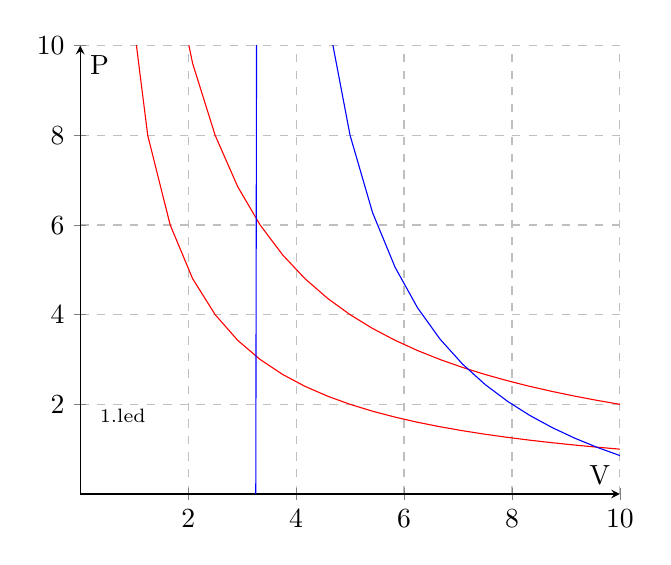
\begin{tikzpicture}
	\begin{axis}[
	    xlabel={V},
	    ylabel={P},
	    xmin=0, xmax=10,
	    ymin=0, ymax=10,
	    xtick={0,2,4,6,8,10},
	    ytick={0,2,4,6,8,10},
	    ymajorgrids=true,
	    xmajorgrids=true,
	    grid style=dashed,
	    axis lines=middle,
	]
	\addplot[domain=0:10,red] {10/(x) };
	\addplot[domain=0:10,red] {20/(x)};
	\addplot[domain=0:10,blue] {20/(x-3) - 2};


	\end{axis}

	\node[text width=1cm] at (0.75,1){\scriptsize {1.led}};

\end{tikzpicture}